\def\notedate{2023.02.01}
\def\currentauthor{Журавлев Н.В. (РК6-72Б), Соколов А.П.}
\notestatement{rndhpcedt}{Алгоритм обхода орграфа, описывающего графовую модель сложного вычислительного метода}

Далее используется терминология, введённая в работах \cite{SokPersh2019PCS, SokGolub2021GBSEBL}.  

\begin{task}
Дано: ориентированный граф $G$ (орграф), возможно, содержащий циклы, определённый множествами узлов $\{S_i\}_1^m$ и рёбер $\{e_{ij}\colon i\in[1\ldotp\ldotp M], j\in[1\ldotp\ldotp N]\}$, где $M,N$ -- некоторые целые числа.\\
Требуется: разработать алгоритм обхода орграфа $G$, который описывает графовую модель некоторого сложного вычислительного метода (СВМ)~\cite{SokPersh2019PCS}. Алгоритм должен учитывать, что в некоторых узлах могут быть определены условия перехода от узла к узлу с помощью понятия функция-селектор~\cite{SokGolub2021GBSEBL}.
\end{task}

Рассмотрим некоторый узел $S_i$ орграфа $G$, из которого выходит множество рёбер $E_i=\{e_{ij}\}_1^n$, $n>0$. Для построения алгоритма обхода необходимо определить правила перехода от узла $S_{i}$ к другим узлам.
\begin{enumerate}
  \item Если $n=1$, то переход безусловный, т.е. предполагает вызов связанной с $e_{ij}$ функции перехода $F_{ij}$, где $j$ соответствует номеру следующего узла $S_j$.
  \item Если $n>1$, то переход следует осуществлять по всем рёбрам, которые определяются с помощью функции-селектора $h_i$ (организует ветвление, рис.~\ref{rndhpcedt.20230201.1}), сопоставленной с узлом $S_i$, результат выполнения которой определяет подмножество $\hat{E}_i=\{a_{ik}\colon {a_{ik}\in E_i}, {\pr_k(h_i(D_i))=1}, {D_i \filledemptyspoon S_i}\}$, где $S_i$ -- состояние данных \gls{ccm}, сопоставленное с одноимённым узлом $S_{i}$, $D_i$ -- данные в состоянии $S_i$, $\pr_{i}(r)$ -- операция проекции объекта $r$ на $i$-ю координату. Порядок выбора рёбер из $\hat{E}_i$ для осуществления перехода не важен.
\end{enumerate}

\begin{figure}[!ht]
	\centering
	\def\udoffset{10mm}
	\tikzstyle{ar} = [->, >={Stealth[length=8pt]}]
	\tikzstyle{tx} = [midway,sloped,anchor=center, above]
	\begin{tikzpicture}[node distance=2.8cm, scale=1.4]
		\node[state] (S) [xshift=-10mm] {$S_i, h_i$};
		\node[state] (S0) [left of=S] {$\cdots$};
		\node (Sm1) [left of=S0] {$\cdots$};
		\draw [ar] (Sm1) -- (S0);
		\draw [ar] (S0) -- (S);
		\node[state] (S1) [above right of=S, xshift=5mm] {$S_1$};
		\node[state] (S2) [right of=S, xshift=5mm] {$S_2$};
		\node (S11) [right of=S1, xshift=-5mm] {$\cdots$};
		\node (S12) [right of=S2, xshift=-5mm] {$\cdots$};
		\draw [dashed,ar] (S) -- node [tx] {\small $e_{i1}, b_1=1$} (S1);
		\draw [ar] (S1) -- (S11);
		\draw [dashed,ar] (S) -- node [tx] {\small $e_{i2}, b_2=0$} (S2);
		\draw [ar] (S2) -- (S12);
		\draw [dashed,ar] (S) .. controls +(north:1.25*\udoffset) and +(north:1.25*\udoffset) .. node [tx] {\small $e_{i3}, b_3=0$} (S0);
	\end{tikzpicture}
	\caption{Организация ветвления с помощью функции-селектора $h_i$ из состояния $S_i$, где $\forall D_i\filledemptyspoon S_i\rightrightarrows\{S_j\}_{j=1}^{n}$ и $h_i(D_i)=\mbf{b}=(b_1,b_2,b_3,\ldots,b_n)=(1,0,0,\ldots)$. Очевидно, что для представленной иллюстрации $\hat{E}_i=\{e_{i1}\}$ и переход по ветвям, для которых $b_i=0$, запрещён}
	\label{rndhpcedt.20230201.1}
\end{figure}

\begin{remark}
Реализация $\hat{E}_i$ для каждого $i$ возможна путём формирования структуры данных стек. Заполнение соответствующего стека элементами может быть осуществлено в произвольном порядке\footnote{Должны быть выполнены все функции перехода $F_{ij}$, связанные с соответствующими рёбрами, в произвольном порядке (возможно в многопоточном режиме).}.
\end{remark}

Для реализации требуемого алгоритма необходимо: сделать класс дуги и в класс узла добавить поля, которые определяют необходимое число для перехода через данный узел и количество дуг, которые уже пришли в узел. Класс дуги содержит два поля: начальный узел и конечный узел.

Рассмотрим работу алгоритма на примере орграфа, представленного на рисунке~\ref{fig:graph}. Начальная вершина называется \textsf{Start}, а конечная \textsf{End}. Селекторы в данном примере отсутствуют.%, однако, их добавление не помешает корректной работе алгоритма.

\begin{figure}[h]
    \centering
    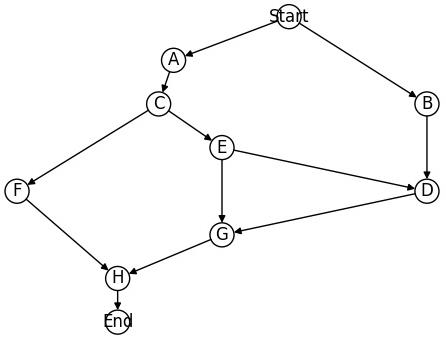
\includegraphics[width=0.55\linewidth]{ResearchNotes/rndhpc_alg_edt_2023_02_01/graph.jpg}
    \caption{Пример орграфа без циклов}
    \label{fig:graph}
\end{figure}

Рассмотрим алгоритм перехода из узла \textsf{Start}. Так как из узла \textsf{Start} выходит два ребра, то выбираем случайное из них (например, ребро \textsf{Start$\rightarrow$A}), совершаем соответствующий переход\footnote{Выполняем соответствующую функцию перехода при \flqq боевом \frqq режиме обхода.}, тогда как оставшееся ребро \textsf{Start$\rightarrow$B} заносится в стек.\messnote{Может быть в любом случае формировать стек?} После перехода в \textsf{A}.  Затем из-за того, что всего доступна только одна вершина, переход происходит в вершину \textsf{C}.

Далее происходит ситуация, что из вершины опять выходит два ребра. Аналогичным образом для перехода выбираем, например, ребро \textsf{C$\rightarrow$E}, тогда в стек заносится ребро \textsf{C$\rightarrow$F}. После выполнения перехода в вершину \textsf{E} ещё раз необходимо выполнение таких же действий. Допустим переход осуществляется по ребру \textsf{E$\rightarrow$D}, а \textsf{E$\rightarrow$G} заносится в стек. На текущий момент в стеке находится три ребра - \textsf{Start$\rightarrow$B}, \textsf{C$\rightarrow$F}, \textsf{E$\rightarrow$G}.

После выполнения перехода в вершину \textsf{D} оказывается, что она требует для продолжения выполнение перехода ещё по ребру \textsf{B$\rightarrow$D}. Следовательно, из стека достаётся ребро - \textsf{E$\rightarrow$G} и осуществляется переход по данному ребру. Далее, при попытке переход через вершину \textsf{G} получается, что необходимо выполнения ребра \textsf{D$\rightarrow$G}, достаётся следующее ребро из стека. Далее выполняется переход по ребру \textsf{C$\rightarrow$F}. Аналогично переход по ребру \textsf{F$\rightarrow$H}. Далее вершина \textsf{H} для продолжения обхода требует переход по \textsf{G$\rightarrow$H}. Из-за этого берется ребро из стека и выполняется переход по нему.

Затем, после перехода по ребру \textsf{B$\rightarrow$D}, в вершине \textsf{D} проверяется разрешается ли переход далее. Так как все нужные для продолжения обхода ребра уже пройдены, то переход разрешается. Далее из этой вершины по ребру \textsf{D$\rightarrow$G} осуществляется переход. В вершине \textsf{G} повторяется аналогичная ситуация, поэтому осуществляется переход по ребру \textsf{G$\rightarrow$H}. Далее по такому же правилу алгоритм доходит до вершины \textsf{End}, чем заканчивает обход.

\noteattributes{} 